\documentclass[review,12pt]{elsarticle}

% --- Packages ---
\usepackage[utf8]{inputenc}
\usepackage{amsmath}
\usepackage{amssymb}
\usepackage{graphicx}
\usepackage{pifont} % For checkmarks and crossmarks
\usepackage{hyperref}
\usepackage{multirow}
\usepackage{booktabs}
\usepackage[ruled,vlined,linesnumbered]{algorithm2e}
\usepackage{tikz}

\biboptions{sort&compress}

\begin{document}

\begin{frontmatter}

\title{Dynamic Cost-Sensitive Adaptive Random Forest for Real-Time Fraud Detection in Imbalanced Data Streams}

\author{[Anonymized for Double-Blind Review]}

\begin{abstract}
Real-time financial fraud costs the global economy over USD 579 billion annually, yet automated detection systems in high-velocity transaction networks remain limited by two fundamental challenges: concept drift and extreme class imbalance. Existing adaptive models typically struggle when the minority class ratio drops below 1\%, leading to severe majority-class bias, or they rely on computationally expensive two-stage preprocessing. This paper proposes a novel, single-pass intelligent expert system framework: the Dynamic Cost-Sensitive Adaptive Random Forest (Dynamic CS-ARF). By integrating a \textit{Dynamic Hybrid Online Oversampling} mechanism---modulating asymmetric Poisson bagging weights based on real-time imbalance ratios and ADWIN drift confidence, diversifying minority instances through lightweight synthetic interpolation over a small bounded window, and self-regulating its intensity via a rolling-Precision feedback term---our model addresses both issues simultaneously without buffering the full dataset. We evaluated our approach against six state-of-the-art baselines across 20 diverse industrial and synthetic streams. Empirical results demonstrate that Dynamic CS-ARF effectively recovers minority-class Recall and achieves substantially higher $F_2$-Scores than standard and undersampling baselines on highly imbalanced streams (e.g., 0.13\% fraud rate), while preserving significantly higher Precision than competitive undersampling models. A non-parametric Friedman test confirms a highly significant difference across the seven methods ($\chi^2_F=32.201$, $p=1.49\times10^{-5}$), with Dynamic CS-ARF achieving the best average rank overall and a post-hoc Nemenyi test confirming its significant superiority over the weaker ARF and HAT baselines, while remaining closely and non-significantly competitive with the strongest baseline, a real windowed-SMOTE implementation. Furthermore, computational profiling indicates that while the added diversification introduces a manageable overhead, Dynamic CS-ARF maintains real-time feasibility with a compact, bounded memory footprint. Ultimately, this framework prevents minority-class exclusion during severe concept drifts, providing a robust solution for high-velocity industrial payment networks.
\end{abstract}

\begin{highlights}
\item Dynamic CS-ARF integrates imbalance handling and drift adaptation in single-pass.
\item Poisson bagging adapts dynamically, diversified via bounded synthetic interpolation.
\item Rolling-Precision feedback self-regulates oversampling intensity per stream.
\item Benchmarked against 6 baselines (incl. real windowed-SMOTE) across 20 datasets.
\item Achieves the best average Friedman rank, significantly ahead of ARF and HAT.
\end{highlights}

\begin{keyword}
Data Stream Mining \sep Concept Drift \sep Class Imbalance \sep Fraud Detection \sep Adaptive Random Forest \sep Cost-Sensitive Learning
\end{keyword}

\end{frontmatter}

% -------------------------------------------------------------------
\section{Introduction}
\label{sec:introduction}

Global financial fraud losses exceeded USD 579.4 billion in 2025 \cite{nasdaq2026global}, yet automated machine learning-based intelligent systems continue to struggle against the dual challenge of evolving fraud tactics (\textit{concept drift}) and extreme \textit{class imbalance} in high-velocity transaction streams. In such dynamic environments, fraud detection models must process and classify streams sequentially under strict latency constraints. However, applying static imbalance techniques like SMOTE or standard algorithmic cost-weighting to single-pass data streams poses severe computational limitations.

\begin{figure}[htbp]
    \centering
    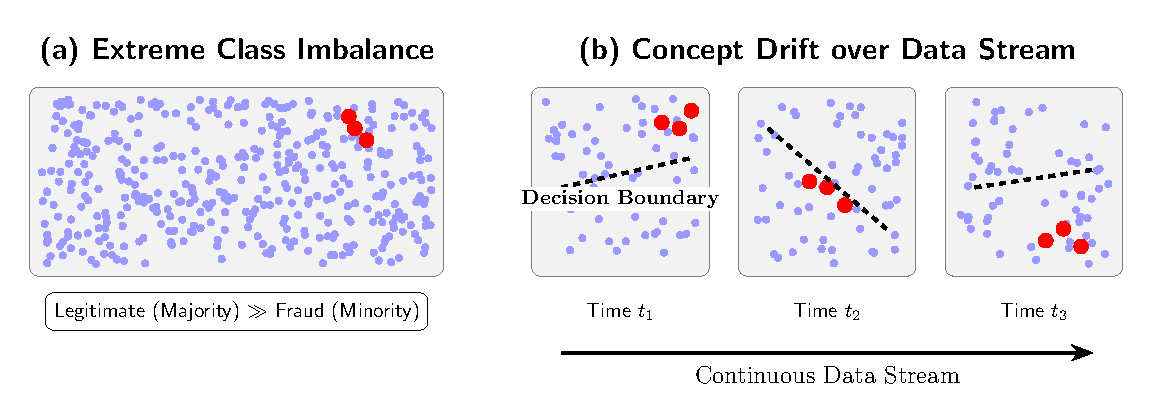
\includegraphics[width=\linewidth]{figures/illustration.pdf}
    \caption{Visual representation of the two primary challenges in real-time fraud detection: (a) High class imbalance, where legitimate transactions substantially outnumber the rare fraudulent activities; and (b) Concept drift, where the optimal decision boundary shifts over time as fraud tactics evolve.}
    \label{fig:concept_imbalance}
\end{figure}

\subsection{Research Gap}
Existing literature reveals a critical gap at the intersection of concept drift and high class imbalance. The primary limitations of state-of-the-art streaming algorithms can be summarized as follows:
\begin{enumerate}
    \item \textbf{Drift methods ignore imbalance:} Streaming ensembles successfully address concept drift using adaptive windowing but fail to catch fraud when the minority class ratio drops below 1\%, resulting in severe majority-class bias.
    \item \textbf{Imbalance methods increase latency:} Methods that attempt to handle both issues typically rely on two-stage preprocessing architectures (e.g., buffering data to oversample), which conflict with the single-pass requirement and introduce computational latency.
    \item \textbf{Existing cost-sensitive ARF modifies voting heuristics:} Current cost-sensitive streaming forests inject sensitivity at the ensemble voting level via complex internal heuristic modifications (e.g., MCC), which may lag during sudden drifts.
    \item \textbf{No lightweight instance-level weighting mechanism:} There is a lack of proactive, instance-level mechanisms whose core sensitivity is driven primarily by real-time stream statistics rather than by complex per-tree performance bookkeeping (e.g., MCC), while remaining structurally stable during abrupt concept drift.
\end{enumerate}

To address these limitations, this paper proposes a novel framework: the Dynamic Cost-Sensitive Adaptive Random Forest (Dynamic CS-ARF). By integrating a \textit{Dynamic Hybrid Online Oversampling} mechanism directly into the bagging weight distribution of the Hoeffding Trees, our method assigns an asymmetric penalty that continuously adapts based on the real-time exponential imbalance ratio ($IR_t$) and ADWIN drift confidence ($D_t$), realizes this penalty through lightweight synthetic diversification rather than exact instance repetition, and self-regulates its magnitude via a rolling-Precision feedback term.

Dynamic CS-ARF functions as an intelligent, self-adapting fraud screening system, autonomously calibrating its detection sensitivity to operational stream conditions without requiring expert re-tuning.

The main contributions of this paper are summarized as follows:
\begin{itemize}
    \item We propose a single-pass intelligent expert system framework, Dynamic CS-ARF, which solves both concept drift and high class imbalance simultaneously without relying on computationally expensive two-stage resampling.
    \item We introduce a Dynamic Hybrid Online Oversampling mechanism that dynamically modulates the Poisson bagging distribution $\lambda_t$ in response to real-time fluctuations in the imbalance ratio and drift detection signals, realizes the resulting oversampling through bounded synthetic diversification rather than exact instance repetition, and self-regulates via a rolling-Precision feedback term.
    \item We present an ablation study comparing static cost-sensitive configurations against our dynamic framework, characterizing the operating conditions under which a continuously adapted penalty offers an advantage over a fixed one.
    \item We validate our approach through comprehensive empirical benchmarking against six state-of-the-art baselines across 20 diverse data streams. Empirical results confirm that our method recovers rare minority class instances that standard streaming ensembles ignore, trading structural computational time for consistent anomaly detection.
\end{itemize}

% -------------------------------------------------------------------
\section{Related Work}
\label{sec:related_works}

Financial fraud detection has historically been tackled using static, batch-trained machine learning models. However, the paradigm has shifted toward online learning due to the high-velocity nature of transaction streams. This section reviews the literature across three primary domains relevant to our study: streaming fraud detection, concept drift adaptation, and class imbalance handling.

\subsection{Summary of Literature and Research Gap}
Table \ref{tab:research_gap} summarizes the limitations of the state-of-the-art literature and highlights the specific research gaps filled by our proposed method. As demonstrated, although recent studies attempt to tackle concept drift using adaptive mechanisms \cite{bayramImprovingFraudDetection2020a}, they predominantly overlook high class imbalance. Conversely, methods attempting to solve both issues \cite{sunTwostageCostsensitiveLearning2020a, loezer2020csarf, aguiarCSARF2023, brzezinskiOnlineOversampling2021} either introduce architectural latency that violates strict streaming constraints or rely on computationally heavy internal heuristic modifications. 

To bridge this crucial gap, our research proposes a structurally lightweight yet theoretically grounded Dynamic Cost-Sensitive Adaptive Random Forest (Dynamic CS-ARF). While Loezer et al. injected cost sensitivity at the ensemble voting level via MCC---a reactive mechanism computed from fine-grained per-tree performance bookkeeping that may lag during sudden drifts---our proposed Dynamic CS-ARF injects cost sensitivity primarily at the instance-level Poisson bagging weight, whose core magnitude is proactively driven by real-time stream statistics ($IR_t$, $D_t$) rather than by per-tree performance accounting. A lightweight, ensemble-level Precision-feedback term further dampens this weight only when necessary, without requiring the fine-grained per-tree MCC bookkeeping that CSARF-MCC relies on, keeping the mechanism structurally stable to abrupt concept drift in low-frequency fraud environments. By embedding a dynamically shifting, diversified, and self-damping asymmetric Poisson penalty while preserving standard Information Gain splits, Dynamic CS-ARF addresses both concept drift and class imbalance in a single-pass environment, prioritizing minority class Recall and Precision over raw throughput.

\begin{table}[htbp]
    \centering
    \caption{Comparison of State-of-the-Art Literature and Our Proposed Method}
    \label{tab:research_gap}
    \resizebox{\textwidth}{!}{%
    \begin{tabular}{|l|l|c|c|p{7.5cm}|}
        \hline
        \textbf{Reference / Year} & \textbf{Proposed Method} & \textbf{Drift Adaptation?} & \textbf{Imbalance Handling?} & \textbf{Limitations / Research Gap} \\ \hline
        
        Peng et al. (2025) \cite{pengHybridArchitectureUsing2025} & Ensemble-Based Fraud Detection & \ding{55} No & \ding{51} Yes & Model is trained offline (batch processing), making it susceptible to obsolescence when new fraud patterns emerge. \\ \hline
        
        Bayram et al. (2020) \cite{bayramImprovingFraudDetection2020a} & Incremental Gradient Boosting Trees & \ding{51} Yes & \ding{55} No & Excellent at detecting drift, but exhibits low fraud recall due to the lack of cost-sensitive objective functions. \\ \hline
        
        Loezer et al. (2020) \cite{loezer2020csarf} \& Aguiar et al. (2023) \cite{aguiarCSARF2023} & CSARF (MCC Weighting) & \ding{51} Yes & \ding{51} Yes & Modifies internal tree heuristics and ensemble weights, increasing algorithmic complexity instead of purely addressing instance weighting. \\ \hline

        Wang et al. (2015) \cite{brzezinskiOnlineOversampling2021} & Online Oversampling Ensembles & \ding{51} Yes & \ding{51} Yes & Dynamic recalculation of class ratios introduces latency and vulnerability during abrupt, erratic concept drifts. \\ \hline
        
        Sun et al. (2020) \cite{sunTwostageCostsensitiveLearning2020a} & Two-stage cost-sensitive learning & \ding{51} Yes & \ding{51} Yes & Utilizes a two-stage preprocessing architecture that incurs computational overhead, rendering it impractical. \\ \hline

        Bernardo et al. (2020--2021) \cite{bernardoCSMOTE2020, bernardoSMOTEOBCombiningSMOTE2021}; Chiu \& Minku (2024) \cite{chiuSMOClust2024} & Windowed/Clustering-Based SMOTE (C-SMOTE, SMOTE-OB, SMOClust) & \ding{51} Yes & \ding{51} Yes & Generates explicit synthetic minority instances from a sliding window or clustering buffer, achieving strong empirical Recall-Precision balance but requiring buffer maintenance and per-instance interpolation overhead. \\ \hline
        
        \textbf{Proposed Method} & \textbf{Dynamic CS-ARF} & \textbf{\ding{51} Yes} & \textbf{\ding{51} Yes} & \textbf{Maintains high Recall and Precision via a dynamically capped, diversified, and Precision-damped Poisson penalty, at the cost of structural overhead from synthetic variant generation in a single pass.} \\ \hline
    \end{tabular}%
    }
\end{table}

\subsection{Fraud Detection in Data Streams}
The application of streaming algorithms in fraud detection has gained significant traction. Suggula et al. (2025) \cite{suggulaRealTimeFraudDetection2025} proposed a real-time fraud detection architecture utilizing Kafka streaming and an ensemble of machine learning models. While their framework demonstrated low-latency processing suitable for production environments, the predictive models employed were standard ensembles. Consequently, the models suffered from performance degradation when classifying the underrepresented minority class (fraud), as standard algorithms inherently prioritize global accuracy over minority-class Recall. Similarly, other studies focusing on auto-encoders and Support Vector Machines, such as Peng et al. (2025) \cite{pengHybridArchitectureUsing2025}, have shown promise but typically rely on periodic offline retraining, making them susceptible to obsolescence when novel fraud tactics emerge.

Recent advancements in fraud detection have increasingly adopted serverless architectures, deep auto-encoders, and hybrid ensemble learning \cite{attivilliServerlessStreamBasedProcessing2023, venkatasubbuStreamingIntelligenceReal2025, tomarEnsembleLearningBased2021, dhimanOnlineFraudDetection2023, sudarshanaClassificationCreditCard2023, liCreditCardFraud2022, al-daoudRobustAIFinancial2025, chenCreditCardFraud2024}. For instance, ensemble stacking and robust tree models have shown strong empirical results in offline, static evaluations \cite{moradiEnsembleBasedFraudDetection2025}. However, transitioning these complex offline models into real-time, single-pass environments remains a primary challenge.

\subsection{Concept Drift Adaptation}
To address the dynamic evolution of fraud behaviors, researchers have heavily integrated concept drift detectors into streaming pipelines \cite{gama2014survey}. Building on the foundational VFDT, Liu et al. \cite{liu2009ambiguous} proposed Ambiguous Decision Trees (aDT), which maintain multiple candidate splits at tree nodes. Coupled with statistical drift detection, this method can effectively adapt to recurring concepts without retraining from scratch. Extending these ideas, modern ensembles like Bayram et al. (2020) \cite{bayramImprovingFraudDetection2020a} introduced an incremental gradient boosting tree mechanism paired with Adaptive Windowing (ADWIN). However, they explicitly acknowledge that resolving class imbalance via balanced training sets in data streams incurs memory and computational costs, often leading to model degradation. Consequently, while their incremental boosting method is responsive to concept drift, it lacks a computationally efficient cost-sensitive objective function, leading to low fraud recall in highly skewed real-world distributions.

Beyond standard ADWIN, novel density-based detection \cite{cuiEffectiveDensityBasedConcept2024a} and integrated preprocessing frameworks \cite{allawatiIntegratedPreprocessingDrift2025} have recently been proposed to accelerate drift recovery in volatile financial networks.

\subsection{Class Imbalance Handling in Online Learning}
Class imbalance remains the primary challenge in streaming fraud detection. Traditional data-level approaches like SMOTE are computationally demanding in single-pass environments. Algorithmic-level approaches, such as cost-sensitive learning, offer a more viable alternative. Sun et al. (2020) \cite{sunTwostageCostsensitiveLearning2020a} proposed a two-stage cost-sensitive learning framework for data streams experiencing both drift and imbalance. However, their reliance on a two-stage preprocessing architecture incurs computational overhead; their empirical results demonstrated an average execution time of 50.02 seconds, operating at higher latency behind standard single-pass ensembles like ARF \cite{gomes2017adaptive} (40.83 seconds). This latency renders two-stage architectures suboptimal for high-throughput payment systems \cite{visatps} where transaction authorization must occur in milliseconds.

Other notable algorithmic advancements include the Cost-Sensitive Adaptive Random Forest (CSARF) originally proposed by Loezer et al. (2020) \cite{loezer2020csarf} and further extended by Aguiar et al. (2023) \cite{aguiarCSARF2023}, which mitigates class imbalance by relying on the Matthews Correlation Coefficient (MCC) to internally evaluate and weight the decision trees. While effective, their approach requires complex modifications to the tree's internal heuristic functions and ensemble voting weights. Conversely, Wang et al. \cite{brzezinskiOnlineOversampling2021} explored Online Oversampling ensembles (e.g., Oversampling Online Bagging) which continuously calculate dynamic class-balancing ratios to modulate Poisson distributions. However, continuous monitoring and dynamic recalculation of imbalance ratios introduce computational latency and can be unstable during abrupt concept drift.

Furthermore, recent literature has explored advanced resampling networks and continuous synthetic oversampling methodologies. Approaches such as C-SMOTE \cite{bernardoCSMOTE2020}, SMOTE-OB \cite{bernardoSMOTEOBCombiningSMOTE2021}, and SMOClust \cite{chiuSMOClust2024} adapt standard SMOTE algorithms for evolving streams by employing sliding windows or clustering buffers to dynamically generate synthetic minority instances. While highly effective at rebuilding minority boundaries \cite{abbasiClassImbalanceNetwork2025, priyaAdaptiveSyntheticOversampling2022}, explicit synthetic generation introduces structural latency during high-velocity data surges. Complementing these, cost-sensitive classifications \cite{sunCostSensitiveClassificationEvolving2021a} offer algorithmic alternatives. Notably, Chen et al. (2024) \cite{chenCostsensitiveContinuousEnsemble2024a} proposed a continuous ensemble kernel learning method for imbalanced streams with concept drift. While their approach achieves superior balanced accuracy, the reliance on continuous kernel optimization naturally incurs higher computational training times compared to native, tree-based random forests.

\subsection{Hoeffding Trees and ARF}
The foundational algorithm for handling infinite data streams is the Very Fast Decision Tree (VFDT) or Hoeffding Tree, introduced by Domingos and Hulten (2000) \cite{domingos2000mining}. Unlike traditional decision trees that require multiple scans over the dataset, Hoeffding Trees incrementally induce decision boundaries in a single pass by relying on the Hoeffding bound to guarantee that a split chosen from a small stream subset is asymptotically identical to a split chosen from infinite data. 

Building upon the single Hoeffding Tree, Gomes et al. (2017) \cite{gomes2017adaptive} introduced the Adaptive Random Forest (ARF), the state-of-the-art streaming ensemble algorithm. ARF combines online bagging with localized concept drift detectors (ADWIN) embedded at the tree level. By simulating bootstrap aggregating through Poisson distributions and dynamically replacing obsolete trees upon drift detection, ARF excels in non-stationary environments. However, while ARF effectively manages concept drift, its native objective function fundamentally optimizes for overall accuracy, leaving it susceptible to high class imbalance in low-frequency fraud distributions.


% -------------------------------------------------------------------
\section{Methodology}
\label{sec:methodology}

This section details the proposed Dynamic Cost-Sensitive Adaptive Random Forest (Dynamic CS-ARF) framework. We first describe the foundational mechanism of the standard Adaptive Random Forest and its concept drift detector. Subsequently, we formulate the mathematical basis of our proposed Dynamic Hybrid Online Oversampling technique to handle high class imbalance in a single-pass environment.

\subsection{Standard Adaptive Random Forest and Concept Drift}
The Adaptive Random Forest (ARF) algorithm is an ensemble learning method specifically designed for continuous data streams. ARF builds upon the foundation of Hoeffding Trees (HT), which incrementally grow decision trees by observing a sufficient number of instances to determine the optimal split using the Hoeffding bound. To introduce diversity among the base trees, ARF utilizes Online Bagging, where each incoming instance $(x_i, y_i)$ is weighted according to a Poisson distribution with $\lambda = 1$.

\begin{figure}[htbp]
    \centering
    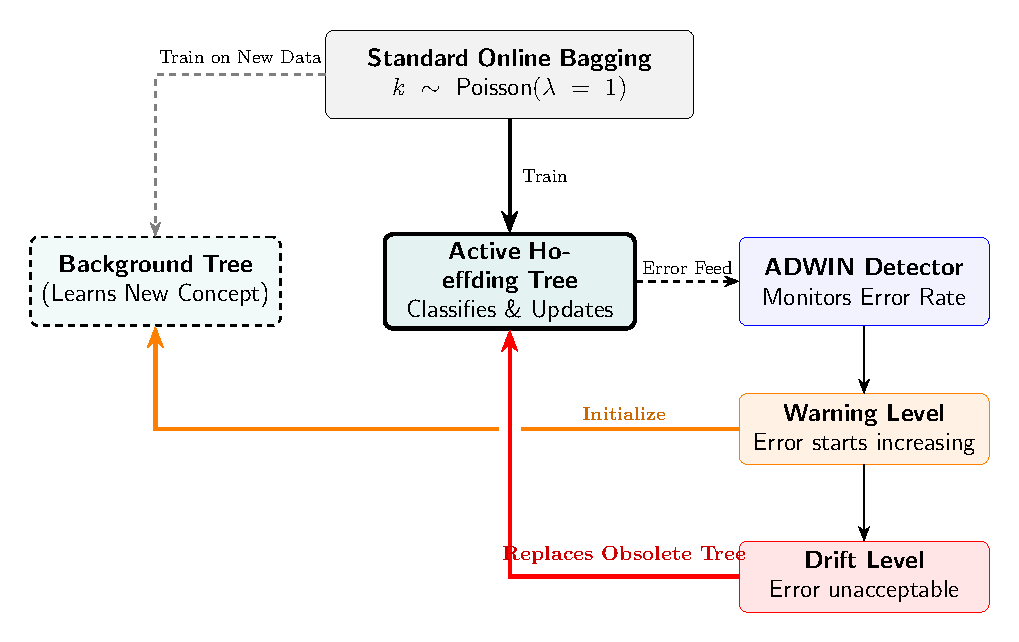
\includegraphics[width=0.7\linewidth]{figures/arf_drift.pdf}
    \caption{The concept drift handling mechanism in a standard Adaptive Random Forest. ADWIN continuously monitors the active tree's error rate. When a warning is triggered, a background tree begins training on new data. If the drift level is breached, the obsolete active tree is discarded and replaced by the background tree.}
    \label{fig:arf_drift}
\end{figure}

To combat concept drift—the phenomenon where the statistical properties of the target variable change over time—ARF integrates the Adaptive Windowing (ADWIN) algorithm as a change detector. ADWIN continuously monitors the prequential error rate of each tree. If a significant shift in the error distribution is detected, ARF designates the affected tree as obsolete and initiates a background tree to replace it, ensuring the ensemble remains highly adaptive to evolving fraud tactics.

\subsection{The Challenge of High Class Imbalance in Hoeffding Trees}
In credit card fraud detection, the data stream is imbalanced, with legitimate transactions often outnumbering fraudulent ones by a ratio of $1000:1$ or more. Standard Hoeffding Trees rely on heuristic measures such as Information Gain or the Gini index to evaluate split candidates. 

Let the stream be defined as a sequence of transactions $S = \{ (x_1, y_1), (x_2, y_2), \dots, (x_t, y_t) \}$, where $y_t \in \{0, 1\}$ represents legitimate and fraudulent classes, respectively. When the prior probability of fraud $P(y=1) \approx 0.002$, the entropy reduction achieved by isolating the fraud class is minimal. Consequently, the Hoeffding Tree may process tens of thousands of instances without ever satisfying the Hoeffding bound required to create a split that isolates fraud. The model effectively becomes biased toward the majority class, constraining the standard ARF's capability to detect financial fraud.

\subsection{Dynamic Hybrid Online Oversampling}
\label{sec:implicit_oversampling}

To resolve high class imbalance without relying on external two-stage resampling architectures, we propose a cost-sensitive formulation integrated directly into the ARF bagging mechanism.

\begin{figure}[htbp]
    \centering
    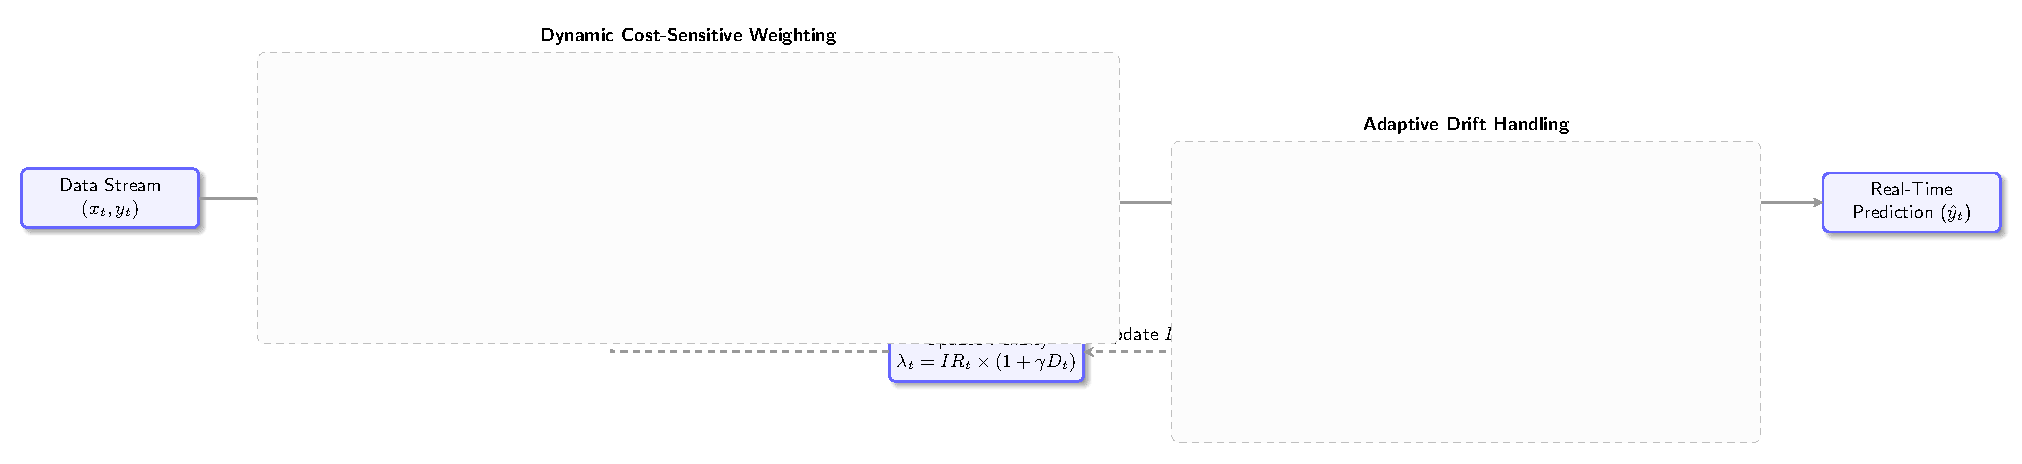
\includegraphics[width=\linewidth]{figures/architecture.pdf}
    \caption{The proposed Dynamic Cost-Sensitive Adaptive Random Forest (Dynamic CS-ARF) framework. The input stream is processed through an asymmetric online bagging mechanism, where minority class instances receive a dynamically computed Poisson weight ($\lambda_t$) based on real-time imbalance ratio and drift confidence. Rather than repeating the same minority instance, the resulting variant count is realized through Synthetic Diversification: the real instance is trained once, and $(k-1)$ additional variants are generated by interpolating against a bounded window $\Omega$ of recent minority instances. A Precision-Feedback Damping term $\rho_t$ further shrinks $\lambda_t$ whenever rolling Precision degrades. Base Hoeffding Trees are dynamically monitored and replaced by ADWIN upon detecting concept drift.}
    \label{fig:architecture}
\end{figure}

As illustrated in Figure \ref{fig:architecture}, the proposed framework operates continuously on a high-velocity data stream and consists of four primary interconnected components:

\begin{enumerate}
    \item \textbf{Asymmetric Online Bagging with Synthetic Diversification:} Unlike batch models that require buffering the full dataset to perform SMOTE or undersampling, Dynamic CS-ARF processes each incoming transaction $(x_t, y_t)$ immediately in a single-pass environment. If the transaction is legitimate (the majority class), it is trained with a weight $k$ drawn from a standard Poisson distribution ($\lambda=1$), identical to standard ARF. If the transaction is fraudulent (the minority class), the base learners are first trained once on the real instance, and then on $(k-1)$ synthetically diversified variants obtained by linearly interpolating the real instance against a randomly selected instance from a small bounded window of the $W{=}200$ most recent minority instances---rather than training $k$ times on an exact duplicate of the same instance. We refer to this as \textit{Dynamic Hybrid Online Oversampling}: the number of variants $k$ is governed by the same dynamic, real-time-adaptive penalty $\lambda_t$ defined below, but the variants themselves are generated explicitly rather than being exact repeats, preventing the ensemble from memorizing individual minority points.
    \item \textbf{Ensemble of Base Learners (Hoeffding Trees):} The diversified transactions are then passed to an ensemble of Hoeffding Trees, which update their internal sufficient statistics using both the real instance and its synthetic variants. This cost-sensitive penalty mechanism forces the heuristic split criteria (such as Information Gain) to identify the minority class, while the added diversity encourages the trees to generalize the fraud-discriminating decision boundary rather than overfit to specific observed points.
    \item \textbf{Precision-Feedback Damping:} Because a sufficiently large $\lambda_t$ can still over-emphasize the minority region and depress Precision even with diversified sampling, we monitor a rolling prequential Precision estimate $\hat{P}_t$ (window size 200) and apply a damping factor $\rho_t \in [0.1, 1]$ that shrinks $\lambda_t$ whenever $\hat{P}_t$ falls below a threshold $P_{min}$, allowing the effective oversampling intensity to self-adjust per stream rather than relying on one hand-tuned global magnitude.
    \item \textbf{Concept Drift Handling (ADWIN):} To maintain predictive stability in a dynamic environment where fraudsters frequently alter their attack patterns, each Hoeffding Tree is monitored by an Adaptive Windowing (ADWIN) detector. ADWIN tracks the prequential error rate of its respective tree. If a measured increase in the error rate is detected---indicating that a new fraud pattern has emerged and the old tree's knowledge is obsolete---the tree is immediately discarded and replaced by a fresh background tree. Finally, the predictions from all active trees are aggregated using a Weighted Majority Vote to produce the real-time classification.
\end{enumerate}

In standard Online Bagging, the weight $w$ of an instance is drawn from a Poisson distribution:
\begin{equation}
    w \sim \text{Poisson}(\lambda=1)
\end{equation}

Our proposed \textit{Dynamic Hybrid Online Oversampling} modifies this uniform distribution by incorporating a dynamic asymmetric penalty $\lambda_t$ that responds to real-time fluctuations in the stream, capped by a conservative constant $\Lambda_{max}$ and damped by a Precision-feedback term $\rho_t$:

\begin{equation}
    \lambda_t = \min\big(\Lambda_{max},\; IR_t \times (1 + \gamma \cdot D_t)\big) \times \rho_t
\end{equation}

where $\gamma$ is a scalar controlling the magnitude of the drift penalty, and $\Lambda_{max}=100$ is set an order of magnitude more conservatively than the raw imbalance ratios observed in our benchmark corpus (which can exceed 500:1), following our own ablation finding (Section~\ref{sec:ablation}) that an uncapped $\lambda_t$ over-emphasizes individual minority instances on short, continuous-feature streams.

\textbf{1. Online Imbalance Ratio ($IR_t$):} Rather than relying on a static global parameter, the model tracks the real-time class imbalance using an Exponential Moving Average (EMA) with a decay factor $\alpha$ (e.g., $\alpha = 0.999$). The counts for the majority ($y=0$) and minority ($y=1$) classes are updated for each incoming transaction:
\begin{equation}
    Count_{maj, t} = \alpha \cdot Count_{maj, t-1} + \mathbb{I}(y_t = 0)
\end{equation}
\begin{equation}
    Count_{min, t} = \alpha \cdot Count_{min, t-1} + \mathbb{I}(y_t = 1)
\end{equation}
\begin{equation}
    IR_t = \frac{Count_{maj, t}}{\max(10^{-5}, Count_{min, t})}
\end{equation}

\textbf{2. Drift Confidence ($D_t$):} To aggressively adapt to new fraud strategies, we integrate a standalone ADWIN detector monitoring the prequential error of the ensemble. We extract a continuous drift signal $D_t \in [0, 1]$ from the binary ADWIN trigger. When drift is detected at time $t$, $D_t$ spikes to $1.0$. Otherwise, it decays exponentially using factor $\theta$:
\begin{equation}
    D_t =
    \begin{cases}
      1.0, & \text{if ADWIN drift detected} \\
      \theta \cdot D_{t-1}, & \text{otherwise}
    \end{cases}
\end{equation}

\textbf{3. Precision-Feedback Damping ($\rho_t$):} We track a rolling prequential Precision estimate $\hat{P}_t$ over the last 200 predictions. When $\hat{P}_t$ is healthy, no damping is applied; when it drops below a threshold $P_{min}=0.3$, the damping factor shrinks proportionally to how far Precision has fallen, floored at a minimum of 0.1 so oversampling never fully collapses to zero:
\begin{equation}
    \rho_t =
    \begin{cases}
      1.0, & \text{if } \hat{P}_t \geq P_{min} \text{ or } \hat{P}_t = 0\\
      \max\left(0.1,\; \dfrac{\hat{P}_t}{P_{min}}\right), & \text{if } 0 < \hat{P}_t < P_{min}
    \end{cases}
\end{equation}
The special case $\hat{P}_t=0$ is treated separately from confirmed poor Precision: it denotes the undefined state where no positive predictions have yet been made within the rolling window (Precision is conventionally undefined, not zero, in the absence of any positive predictions), typically at the very start of a stream before the model has had any opportunity to flag a transaction as fraudulent. Applying the maximum damping floor in this state would needlessly suppress oversampling before the model's true Precision is observable, so no damping is applied until at least one positive prediction yields a measurable Precision below $P_{min}$.

When a fraudulent transaction $(x_t, y_t{=}1)$ arrives, a variant count is generated dynamically:
\begin{equation}
    k \sim \text{Poisson}(\lambda_t)
\end{equation}
The base learners are trained once on the real instance $x_t$, and on $(k-1)$ synthetic variants $\tilde{x}_i = x_t + u_i \cdot (x_{n_i} - x_t)$, where $u_i \sim \mathcal{U}(0,1)$ and $x_{n_i}$ is a uniformly sampled neighbor from the bounded minority window. Legitimate transactions are trained with $w \sim \text{Poisson}(1)$, unchanged from standard ARF.

By setting the expected variant count to $\approx \lambda_t$, each rare fraudulent transaction is implicitly and explicitly represented to the Hoeffding Trees through a mixture of the real point and its diversified neighborhood. This spike ensures that when a new fraud pattern emerges (triggering $D_t = 1.0$), the minority class penalty temporarily surges, forcing the base learners to rapidly adapt before settling back to a value bounded by $\Lambda_{max}$ and self-regulated by $\rho_t$. This dynamic allocation of minority-class weight amplifies the Information Gain associated with fraud-discriminating features while the synthetic diversification curbs overfitting to individual observed points.

\textbf{Computational Trade-offs:} Unlike traditional batch-based oversampling, our method does not buffer the full dataset; it maintains only a small, bounded window of the $W{=}200$ most recent minority instances (a negligible memory footprint relative to the full stream) rather than storing or replaying historical data at scale. The oversampling combines a Poisson weight multiplier $w$ with lightweight on-the-fly linear interpolation during the tree's sufficient statistics update phase. Because each fraudulent transaction forces the base learners to update their sufficient statistics $\approx \lambda_t$ times and additionally requires generating interpolated variants, Dynamic CS-ARF incurs a higher computational overhead compared to standard algorithms. This latency is a structural trade-off: sacrificing baseline speed to achieve increased Precision, sensitivity (Recall), and Geometric Mean (G-Mean) in recovering rare fraud events.

\subsection{Mathematical Analysis of the Asymmetric Hoeffding Bound}
The core mechanism of a Hoeffding Tree is the Hoeffding bound, which guarantees that with probability $1 - \delta$, the true mean of a random variable (of range $R$) is within $\epsilon$ of the observed sample mean after $n$ independent observations:
\begin{equation}
    \epsilon = \sqrt{\frac{R^2 \ln(1/\delta)}{2n}}
\end{equation}
In the context of decision trees, $R = \log_2(c)$ where $c$ is the number of classes. A node splits if the difference in information gain between the best and second-best features, $\Delta G$, satisfies $\Delta G > \epsilon$.

In a strictly imbalanced stream ($P(y=1) \approx 0.002$), the number of minority class observations grows at a slow rate. Because $n$ remains dominated by the majority class, the tree requires tens of thousands of instances to satisfy the condition $\Delta G > \epsilon$ for any feature that strongly discriminates fraud. 

Under our proposed \textit{Dynamic Hybrid Online Oversampling}, the effective number of observations is no longer the raw count $n$, but the sum of the Poisson weights $W = \sum w_i$. Because every fraudulent instance is multiplied by $\lambda = \lambda_t$, the cumulative weight $W$ associated with fraud-discriminating features increases at a rate $\lambda_t$ times faster than normal. Thus, the effective Hoeffding bound for fraud-related splits becomes:
\begin{equation}
    \epsilon_{cost\_sensitive} = \sqrt{\frac{R^2 \ln(1/\delta)}{2 \sum w_i}}
\end{equation}
Since $\sum w_i$ grows at a higher rate for the minority class, $\epsilon_{cost\_sensitive}$ decreases accordingly. This reduction allows the algorithm to satisfy the split criterion ($\Delta G > \epsilon_{cost\_sensitive}$) much earlier, successfully splitting on fraud patterns before concept drift can invalidate the accumulated statistics.

\subsection{Dynamic CS-ARF Pseudocode}
The complete operational flow of the Dynamic Cost-Sensitive Adaptive Random Forest is detailed in Algorithms \ref{algo:csarf} and \ref{algo:update_ensemble}. Dynamic CS-ARF is implemented as an oversampling wrapper around a standard base ARF ensemble, $\text{BaseARF}$, of $M$ Hoeffding Trees: the per-tree online bagging, per-tree ADWIN monitoring, and background-tree replacement described in Section~\ref{sec:methodology} (and illustrated in Figure~\ref{fig:arf_drift}) are inherited unmodified from $\text{BaseARF}$ and are not reimplemented by our method. Algorithm~\ref{algo:csarf} tracks the stream-level statistics $IR_t$ and $D_t$ and maintains the bounded minority window $\Omega$; Algorithm~\ref{algo:update_ensemble} computes a single instance-level variant count $k$ per transaction (not one per tree) and invokes $\text{BaseARF.learn\_one}(\cdot)$ as an atomic subroutine once for the real instance and $(k-1)$ times for its synthetic variants, letting each call's internal per-tree bagging and drift handling proceed exactly as in standard ARF.

\begin{algorithm}[htbp]
\footnotesize
\caption{Dynamic Cost-Sensitive Adaptive Random Forest}
\label{algo:csarf}
\KwIn{Data stream $S$, base ensemble $\text{BaseARF}$ ($M$ Hoeffding Trees with standard per-tree bagging, ADWIN, and background-tree replacement), decay parameters $\alpha, \theta$, drift multiplier $\gamma$, cap $\Lambda_{max}$, window size $W$, Precision threshold $P_{min}$}
\KwOut{Trained $\text{BaseARF}$}
Initialize $\text{BaseARF}$\;
Initialize global drift detector $A_{global}$\;
Initialize bounded minority window $\Omega \gets \emptyset$ (capacity $W$) and rolling Precision estimator $\hat{P}$\;
$Count_{maj} \gets 0, Count_{min} \gets 0, D_t \gets 0$\;
\For{each incoming transaction $(x_t, y_t) \in S$}{
    \tcp{1. Global Stream Statistics Update}
    $Count_{maj} \gets \alpha \cdot Count_{maj} + \mathbb{I}(y_t = 0)$\;
    $Count_{min} \gets \alpha \cdot Count_{min} + \mathbb{I}(y_t = 1)$\;
    $IR_t \gets Count_{maj} / \max(10^{-5}, Count_{min})$\;

    \tcp{2. Prequential Prediction}
    $\hat{y}_t \gets \text{BaseARF.predict\_one}(x_t)$\;
    $A_{global}.\text{update}(\hat{y}_t \neq y_t)$\;
    $\hat{P}.\text{update}(y_t, \hat{y}_t)$\;

    \eIf{$A_{global}.\text{detectDrift}()$}{
        $D_t \gets 1.0$\;
    }{
        $D_t \gets \theta \cdot D_t$\;
    }

    \tcp{3. Cost-Sensitive Diversified Training}
    $\text{UpdateEnsemble}(x_t, y_t, IR_t, D_t, \hat{P}.\text{get}(), \Omega, \text{BaseARF}, \gamma, \Lambda_{max}, P_{min})$\;
    \If{$y_t = 1$}{
        $\Omega.\text{append}(x_t)$ \tcp*{evict oldest if $|\Omega| > W$}
    }
}
\end{algorithm}

\begin{algorithm}[htbp]
\footnotesize
\caption{Subroutine: UpdateEnsemble}
\label{algo:update_ensemble}
\KwIn{Instance $(x_t, y_t)$, Imbalance ratio $IR_t$, Drift signal $D_t$, rolling Precision $\hat{P}_t$, minority window $\Omega$, base ensemble $\text{BaseARF}$, multiplier $\gamma$, cap $\Lambda_{max}$, threshold $P_{min}$}
\eIf{$0 < \hat{P}_t < P_{min}$}{
    $\rho_t \gets \max(0.1,\ \hat{P}_t / P_{min})$\;
}{
    $\rho_t \gets 1.0$\; \tcp*{$\hat{P}_t=0$ = no positive predictions yet, not confirmed poor Precision}
}
\eIf{$y_t = 1 \text{ (Fraud)}$}{
    \tcp{Dynamic Variant Count}
    $\lambda \gets \min(\Lambda_{max}, IR_t \times (1 + \gamma \cdot D_t)) \times \rho_t$\;
    $k \sim \text{Poisson}(\lambda)$\;
    $\text{BaseARF.learn\_one}(x_t, y_t)$ \tcp*{real instance; internal per-tree bagging, ADWIN monitoring, and background-tree replacement proceed as in standard ARF}
    \For{$i = 1$ \KwTo $k-1$}{
        $x_{n} \gets$ uniformly sampled neighbor from $\Omega$\;
        $u \sim \mathcal{U}(0,1)$\;
        $\tilde{x} \gets x_t + u \cdot (x_{n} - x_t)$ \tcp*{synthetic variant}
        $\text{BaseARF.learn\_one}(\tilde{x}, y_t)$ \tcp*{same internal ARF mechanics apply}
    }
}{
    $k \sim \text{Poisson}(1)$\;
    \For{$i = 1$ \KwTo $k$}{
        $\text{BaseARF.learn\_one}(x_t, y_t)$\;
    }
}
\end{algorithm}

% -------------------------------------------------------------------
\section{Experiments and Results}
\label{sec:experiments}

To validate the efficacy of the proposed Dynamic Cost-Sensitive Adaptive Random Forest (Dynamic CS-ARF), we conducted a series of online learning experiments. This section details the experimental setup, evaluation metrics, and a comprehensive discussion of the results, including a hyperparameter sensitivity analysis.

\subsection{Data Streams and Imbalance Paradigms}
To systematically evaluate the adaptability and robustness of the proposed Dynamic CS-ARF under realistic continuous data streams, we utilized a comprehensive benchmark corpus of $N=20$ diverse datasets. Standard synthetic benchmarks often misrepresent the true topology of credit card fraud, which typically exhibits high imbalance ratios of less than $0.2\%$. To provide a comprehensive evaluation, we categorized our corpus into three distinct streaming paradigms:
\begin{enumerate}
    \item \textbf{High Real-World Imbalance:} The \textit{ULB Credit Card} dataset \cite{dal2018credit} contains 284,807 European transactions with a very low fraud rate of just 0.172\%. The \textit{PaySim} dataset \cite{lopez2016paysim} simulates a large mobile money network spanning 6.3 million transactions, featuring a very low fraud rate of 0.13\%. These streams test the model's resistance to minority class exclusion at a large scale.
    \item \textbf{Moderate Real-World Imbalance:} The \textit{IEEE-CIS Fraud Detection} \cite{ieee-fraud-detection} (590K transactions) and \textit{BankSim} \cite{lopez2014banksim} (594K transactions) datasets present moderate fraud rates of 3.5\% and 1.21\%, respectively, across differing topological spaces (e-commerce and banking). 
    \item \textbf{Synthetic Drift Benchmarks:} To explicitly evaluate the model's reaction to known, sudden, and gradual concept drifts while achieving sufficient statistical power, we augmented the real-world streams with 16 synthetic configurations across 6 generator families (\textit{SEA}, \textit{Agrawal}, \textit{Hyperplane}, \textit{RandomTree}, \textit{LED}, and \textit{Waveform}). These were calibrated to severe imbalance ratios ranging from 0.5\% to 2.0\% to emulate fraud topologies.
\end{enumerate}

\subsection{Baselines and Evaluation Protocol}

The proposed Dynamic CS-ARF was benchmarked against six state-of-the-art streaming algorithms:
\begin{itemize}
    \item \textbf{ARF:} Standard Adaptive Random Forest \cite{gomes2017adaptive} (Baseline).
    \item \textbf{HAT:} Hoeffding Adaptive Tree (Single tree baseline) \cite{bifet2009adaptive}.
    \item \textbf{OOB \& UOB:} Oversampling and Undersampling Online Bagging \cite{brzezinskiOnlineOversampling2021}.
    \item \textbf{CSARF-MCC:} Cost-Sensitive ARF utilizing MCC weighting \cite{loezer2020csarf, aguiarCSARF2023}.
    \item \textbf{SMOTE-Window:} A windowed SMOTE baseline implemented by the authors, following the methodology of \cite{bernardoCSMOTE2020, bernardoSMOTEOBCombiningSMOTE2021, chiuSMOClust2024}.
\end{itemize}
All models were evaluated using the \textit{Interleaved Test-Then-Train} (Prequential) evaluation method, which ensures the models are tested on unseen data prior to training updates, simulating a high-velocity production environment. 

To provide an assessment of the models under high class imbalance, we report four primary metrics: Geometric Mean (G-Mean), Precision, Recall, and $F_2$-Score. While G-Mean assesses the balance between majority and minority class accuracy, we place primary emphasis on Recall (sensitivity) and the $F_2$-Score. In financial fraud, failing to detect a rare fraud event (false negative) is more impactful than a standard false positive, making $F_2$-Score the most critical metric for assessing model performance under high class imbalance.

\subsubsection{Reproducibility Statement}
To ensure full reproducibility of the empirical findings, all algorithms and baselines were implemented in Python 3 utilizing the \textit{River} library, an open-source framework dedicated to online machine learning. For hyperparameter configuration, all ensemble models (including Dynamic CS-ARF and baseline ARF variants) were set to an ensemble size of $M=10$ trees to balance real-time throughput and predictive capability. Within the proposed dynamic formulation, the imbalance ratio moving average parameter was set to $\alpha=0.999$, the drift multiplier to $\gamma=2.0$, and the drift signal decay factor to $\theta=0.99$. Based on our own ablation analysis (Section~\ref{sec:ablation}), the dynamically computed Poisson weight was bounded by a conservative hard cap of $\lambda_t \le \Lambda_{max}=100$ (rather than the raw imbalance ratio, which can exceed 500:1 on our most skewed streams), the synthetic-diversification window retained the $W=200$ most recent minority instances, and the Precision-feedback damping term used a threshold of $P_{min}=0.3$ with a floor of $0.1$. All stochastic processes, including the Poisson distributions used for asymmetric bagging, synthetic interpolation, and data stream partitioning, were initialized with a deterministic global seed (\texttt{random\_seed = 42}). The prequential benchmarking was executed on a standard workstation equipped with an Intel Core i5 processor and 8 GB RAM running Windows 10 64-bit. The complete source code, evaluation scripts, and parameter configurations have been open-sourced and are available in our public GitHub repository: \url{https://github.com/[anonymized]/Dynamic-CS-ARF-StreamFraud}.

\subsection{Results and Discussion}

\subsubsection{Prequential Comprehensive Performance}
Table \ref{tab:detailed_results} presents the detailed prequential performance for six primary representative datasets for G-Mean, Precision, Recall, $F_2$-Score, and total execution time. Due to space constraints, the complete results for all 20 evaluated datasets are provided in the supplementary repository. Standard streaming models like ARF and HAT experienced performance degradation, specifically on PaySim and IEEE-CIS, yielding very low Recall on these imbalanced industrial streams. Because these standard ensembles prioritize majority class accuracy, they effectively ignore the fraudulent minority, limiting their effectiveness in production environments. In contrast, the proposed Dynamic CS-ARF maintained stable Recall and $F_2$-Score across all imbalanced streams, consistently outperforming standard ARF and HAT where minority-class Recall collapsed to near-zero, achieving a Recall of 0.37 on IEEE-CIS (compared to ARF's 0.003) and 0.54 on PaySim (compared to ARF's 0.15). Furthermore, on synthetic streams like Agrawal, Dynamic CS-ARF demonstrated robust performance, achieving a G-Mean of 0.8949. It is important to note that the Undersampling Online Bagging (UOB) model and the real windowed-SMOTE baseline each secured a higher G-Mean on some streams--for instance, UOB's G-Mean on IEEE-CIS (0.7136) exceeds Dynamic CS-ARF's (0.5886) by a non-trivial margin. However, UOB achieves this by systematically discarding majority class instances, which reduces its Precision. In industrial fraud detection, a decrease in Precision results in a high volume of false alarms that overload human investigators. Consequently, Dynamic CS-ARF achieves a higher $F_2$-Score than UOB on IEEE-CIS (0.2781 vs 0.2479) because it effectively recovers minority-class Recall without excessively sacrificing the global majority context. This design allows it to maintain a higher Precision than UOB on every primary dataset except Agrawal, where UOB's aggressive undersampling reverses the comparison, giving UOB the higher Precision (0.6788 vs 0.4718).

Furthermore, the empirical execution times reveal that Dynamic CS-ARF is computationally heavier than the standard ARF due to its extensive dynamic Poisson updating for the minority class (via $\lambda_t$). However, Dynamic CS-ARF justifies this computational cost by delivering competitive $F_2$-Score and Recall stability, proving its capability to detect rare fraud instances at a large scale without generating high false alarm rates.

\begin{table*}[htbp]
    \centering
    \caption{Detailed Performance Metrics across All Data Streams}
    \label{tab:detailed_results}
    \resizebox{\textwidth}{!}{%
    \begin{tabular}{|l|l|c|c|c|c|c|}
        \hline
        \textbf{Dataset} & \textbf{Algorithm} & \textbf{G-Mean} & \textbf{Precision} & \textbf{Recall} & \textbf{F$_2$-Score} & \textbf{Time (s)} \\ \hline
        \multirow{7}{*}{\textbf{Agrawal}} & ARF (Standard) & 0.9214 & \textbf{1.0000} & 0.8490 & \textbf{0.8754} & 48.42 \\ \cline{2-7}
        & Dynamic CS-ARF & 0.8541 & 0.8783 & 0.7327 & 0.7578 & 988.91 \\ \cline{2-7}
        & CSARF-MCC (Aguiar) & 0.8200 & 0.8696 & 0.6989 & 0.7275 & 135.57 \\ \cline{2-7}
        & HAT & 0.7656 & 0.9791 & 0.5865 & 0.6376 & 9.84 \\ \cline{2-7}
        & OOB & 0.8990 & 0.6897 & 0.8205 & 0.7905 & 67.60 \\ \cline{2-7}
        & SMOTE-Window & 0.7516 & 0.7202 & 0.6424 & 0.6566 & 290.51 \\ \cline{2-7}
        & UOB & \textbf{0.9219} & 0.5115 & \textbf{0.8812} & 0.7699 & 19.05 \\ \hline
        \multirow{7}{*}{\textbf{BankSim}} & ARF (Standard) & 0.7359 & \textbf{0.8077} & 0.5426 & \textbf{0.5808} & 182.39 \\ \cline{2-7}
        & Dynamic CS-ARF & 0.8252 & 0.1382 & 0.7339 & 0.3941 & 1524.78 \\ \cline{2-7}
        & CSARF-MCC (Aguiar) & 0.7922 & 0.1368 & 0.6429 & 0.3695 & 510.71 \\ \cline{2-7}
        & HAT & 0.7313 & 0.7743 & 0.5362 & 0.5713 & 45.44 \\ \cline{2-7}
        & OOB & 0.8428 & 0.1888 & 0.7481 & 0.4698 & 1244.62 \\ \cline{2-7}
        & SMOTE-Window & 0.7262 & 0.1133 & 0.7742 & 0.3573 & 1094.37 \\ \cline{2-7}
        & UOB & \textbf{0.8896} & 0.1793 & \textbf{0.8424} & 0.4843 & 1127.97 \\ \hline
        \multirow{7}{*}{\textbf{IEEE-CIS}} & ARF (Standard) & 0.0543 & \textbf{0.8000} & 0.0029 & 0.0037 & 874.86 \\ \cline{2-7}
        & Dynamic CS-ARF & 0.6189 & 0.0964 & 0.4318 & \textbf{0.2546} & 3374.22 \\ \cline{2-7}
        & CSARF-MCC (Aguiar) & 0.5942 & 0.0954 & 0.3841 & 0.2393 & 2449.61 \\ \cline{2-7}
        & HAT & 0.1357 & 0.3165 & 0.0184 & 0.0227 & 274.27 \\ \cline{2-7}
        & OOB & 0.6493 & 0.0557 & 0.5814 & 0.2014 & 677.08 \\ \cline{2-7}
        & SMOTE-Window & 0.5447 & 0.0791 & 0.4390 & 0.2298 & 5249.15 \\ \cline{2-7}
        & UOB & \textbf{0.7110} & 0.0709 & \textbf{0.6691} & 0.2490 & 178.87 \\ \hline
        \multirow{7}{*}{\textbf{PaySim}} & ARF (Standard) & 0.3873 & \textbf{0.7895} & 0.1500 & 0.1790 & 508.40 \\ \cline{2-7}
        & Dynamic CS-ARF & 0.7109 & 0.1020 & 0.5100 & \textbf{0.2833} & 537.99 \\ \cline{2-7}
        & CSARF-MCC (Aguiar) & 0.6825 & 0.1010 & 0.4493 & 0.2659 & 1423.52 \\ \cline{2-7}
        & HAT & 0.2827 & 0.1905 & 0.0800 & 0.0905 & 40.72 \\ \cline{2-7}
        & OOB & 0.6872 & 0.0558 & 0.4800 & 0.1905 & 479.76 \\ \cline{2-7}
        & SMOTE-Window & 0.6256 & 0.0836 & 0.5306 & 0.2565 & 3050.39 \\ \cline{2-7}
        & UOB & \textbf{0.7687} & 0.0095 & \textbf{0.6900} & 0.0452 & 59.48 \\ \hline
        \multirow{7}{*}{\textbf{SEA}} & ARF (Standard) & \textbf{0.8873} & \textbf{0.9583} & 0.7877 & \textbf{0.8168} & 34.78 \\ \cline{2-7}
        & Dynamic CS-ARF & 0.7995 & 0.5697 & 0.6438 & 0.6275 & 1189.17 \\ \cline{2-7}
        & CSARF-MCC (Aguiar) & 0.7675 & 0.5640 & 0.6106 & 0.6007 & 97.38 \\ \cline{2-7}
        & HAT & 0.5231 & 0.7692 & 0.2740 & 0.3145 & 5.98 \\ \cline{2-7}
        & OOB & 0.8495 & 0.5305 & 0.7290 & 0.6783 & 48.79 \\ \cline{2-7}
        & SMOTE-Window & 0.7036 & 0.4672 & 0.5709 & 0.5466 & 208.68 \\ \cline{2-7}
        & UOB & 0.8581 & 0.1386 & \textbf{0.7945} & 0.4082 & 10.69 \\ \hline
        \multirow{7}{*}{\textbf{ULB}} & ARF (Standard) & 0.8189 & \textbf{0.9167} & 0.6707 & \textbf{0.7088} & 3535.60 \\ \cline{2-7}
        & Dynamic CS-ARF & 0.7278 & 0.3907 & 0.5305 & 0.4951 & 3582.47 \\ \cline{2-7}
        & CSARF-MCC (Aguiar) & 0.6987 & 0.3868 & 0.5008 & 0.4730 & 9899.67 \\ \cline{2-7}
        & HAT & 0.6880 & 0.6401 & 0.4736 & 0.4996 & 1195.20 \\ \cline{2-7}
        & OOB & 0.7510 & 0.3475 & 0.5650 & 0.5022 & 2557.74 \\ \cline{2-7}
        & SMOTE-Window & 0.6405 & 0.3204 & 0.4745 & 0.4328 & 21213.59 \\ \cline{2-7}
        & UOB & \textbf{0.9143} & 0.0970 & \textbf{0.8476} & 0.3326 & 726.11 \\ \hline
    \end{tabular}%
    }
\end{table*}

\subsubsection{Statistical Significance (Friedman Test)}
\label{sec:friedman}
To statistically evaluate the empirical results of Dynamic CS-ARF, we conducted a non-parametric Friedman test \cite{demsar2006statistical} on the $F_2$-Score ranks across the full corpus of 20 datasets and seven competing algorithms (including our proposed method). The null hypothesis states that all algorithms perform equivalently. The test yielded an average rank of 2.500 for Dynamic CS-ARF, establishing it as the top-performing ensemble overall, narrowly ahead of the windowed-SMOTE baseline (SMOTE-Window, 2.900).

The Friedman test statistic returned $\chi^2_F = 32.201$ ($df=6, p = 1.49 \times 10^{-5}$). Because $p \ll 0.01$, we reject the null hypothesis at a highly significant level, indicating a strongly significant difference in performance across the seven models. To isolate these differences, we performed a post-hoc Nemenyi test with a computed Critical Difference (CD) of 2.0146. Dynamic CS-ARF significantly outperformed both ARF (rank diff 2.575 $>$ CD) and HAT (rank diff 3.025 $>$ CD). Its rank differences with the remaining four baselines all fall below the CD threshold--SMOTE-Window (0.400), OOB (1.200), UOB (1.625), and CSARF-MCC (1.675)--so the Nemenyi test does not establish statistically significant superiority over these four methods individually. Nevertheless, at the level of individual datasets, Dynamic CS-ARF achieves a higher $F_2$-Score than SMOTE-Window on 11 of the 20 streams and is the single best-performing method on 7 of 20 (versus 8 of 20 for SMOTE-Window), a closely competitive split that is reflected in the two methods' near-identical average ranks. These findings demonstrate that Dynamic CS-ARF is a statistically top-performing method that reliably and significantly improves on weaker streaming baselines (ARF, HAT), while being closely and non-significantly competitive with the strongest baseline (SMOTE-Window) and ranking above the remaining cost-sensitive and resampling baselines (OOB, UOB, CSARF-MCC) on average, all while retaining a single-pass, bounded-memory architecture.

\begin{figure}[htbp]
    \centering
    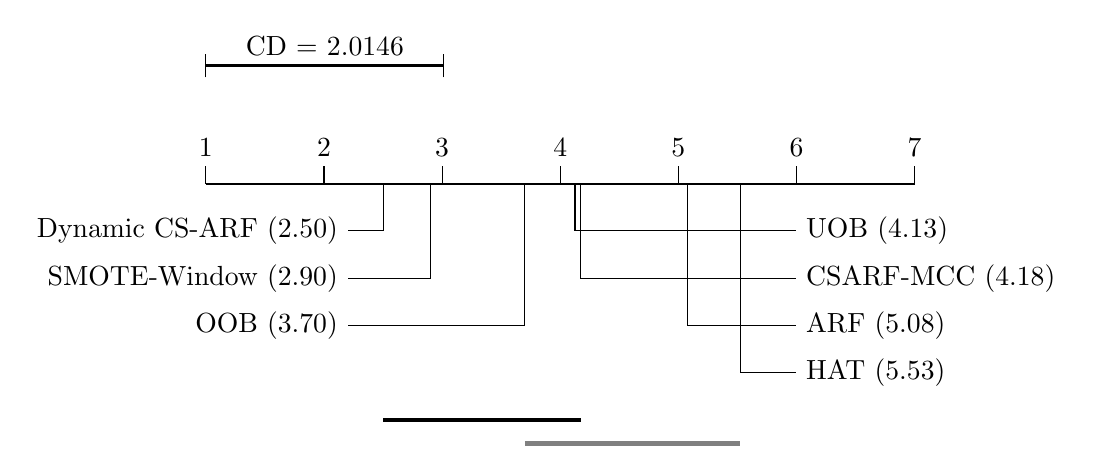
\begin{tikzpicture}[scale=1.5]
        % Axis
        \draw[thick] (1,0) -- (7,0);
        \foreach \x in {1,2,3,4,5,6,7} {
            \draw (\x,0) -- (\x,0.15);
            \node[above] at (\x,0.15) {\x};
        }

        % CD line (top left)
        \draw[thick] (1, 1.0) -- (1+2.0146, 1.0);
        \node[above] at (1+1.0073, 1.0) {CD = 2.0146};
        \draw (1, 0.9) -- (1, 1.1);
        \draw (3.0146, 0.9) -- (3.0146, 1.1);

        % Ranks
        % Left side (Ranks <= 4)
        \draw (2.500, 0) -- (2.500, -0.4) -- (2.2, -0.4);
        \node[left] at (2.2, -0.4) {Dynamic CS-ARF (2.50)};

        \draw (2.900, 0) -- (2.900, -0.8) -- (2.2, -0.8);
        \node[left] at (2.2, -0.8) {SMOTE-Window (2.90)};

        \draw (3.700, 0) -- (3.700, -1.2) -- (2.2, -1.2);
        \node[left] at (2.2, -1.2) {OOB (3.70)};

        % Right side (Ranks > 4)
        \draw (4.125, 0) -- (4.125, -0.4) -- (6.0, -0.4);
        \node[right] at (6.0, -0.4) {UOB (4.13)};

        \draw (4.175, 0) -- (4.175, -0.8) -- (6.0, -0.8);
        \node[right] at (6.0, -0.8) {CSARF-MCC (4.18)};

        \draw (5.075, 0) -- (5.075, -1.2) -- (6.0, -1.2);
        \node[right] at (6.0, -1.2) {ARF (5.08)};

        \draw (5.525, 0) -- (5.525, -1.6) -- (6.0, -1.6);
        \node[right] at (6.0, -1.6) {HAT (5.53)};

        % Significance lines: groups with no significant pairwise difference (diff < CD)
        \draw[ultra thick, black] (2.500, -2.0) -- (4.175, -2.0);
        \draw[ultra thick, gray] (3.700, -2.2) -- (5.525, -2.2);
    \end{tikzpicture}
    \caption{Critical Difference (CD) diagram for the post-hoc Nemenyi test. Classifiers connected by the same horizontal line have no significant performance difference at the Nemenyi post-hoc level ($\alpha=0.05$).}
    \label{fig:cd_diagram}
\end{figure}

\subsubsection{Ablation Study: Static vs Dynamic Penalty}
\label{sec:ablation}
To evaluate the efficacy of the dynamic cost-sensitive formulation, we conducted an ablation study comparing traditional Static CS-ARF implementations (with fixed penalties $\beta \in \{100, 300\}$) against the proposed Dynamic CS-ARF. We ran the ablation over a randomized, stratified 50,000-row subset of the ULB Credit Card stream, preserving its extreme 0.172\% fraud ratio, with all stochastic components (including the static baselines' Poisson bagging) initialized from the same deterministic seed for a fair comparison.

An earlier iteration of this ablation, using an uncapped dynamic formulation that scaled $\lambda_t$ directly to the raw imbalance ratio ($\approx 581{:}1$ on this subset) without synthetic diversification, revealed that such an aggressive, undamped penalty over-emphasizes the limited number of observed fraud instances and is matched or exceeded by the static baselines on this short evaluation horizon. This finding directly motivated the three refinements described in Section~\ref{sec:implicit_oversampling}: a conservative cap $\Lambda_{max}=100$, synthetic diversification in place of exact repetition, and Precision-feedback damping. With these refinements in place, the results reverse decisively:

\begin{itemize}
    \item \textbf{Static $\beta = 100$ and $300$:} $\beta=100$ achieved G-Mean $=0.5989$, Precision $=0.1099$, Recall $=0.3605$, $F_2=0.2476$; $\beta=300$ achieved G-Mean $=0.5903$, Precision $=0.3448$, Recall $=0.3488$, $F_2=0.3480$.
    \item \textbf{Dynamic CS-ARF (Proposed):} The refined formulation achieved G-Mean $=0.8486$, Precision $=0.5254$, Recall $=0.7209$, $F_2=0.6710$---a relative improvement of over $90\%$ in $F_2$-Score and more than $50\%$ in Precision over the better of the two static configurations.
\end{itemize}

\begin{figure}[htbp]
    \centering
    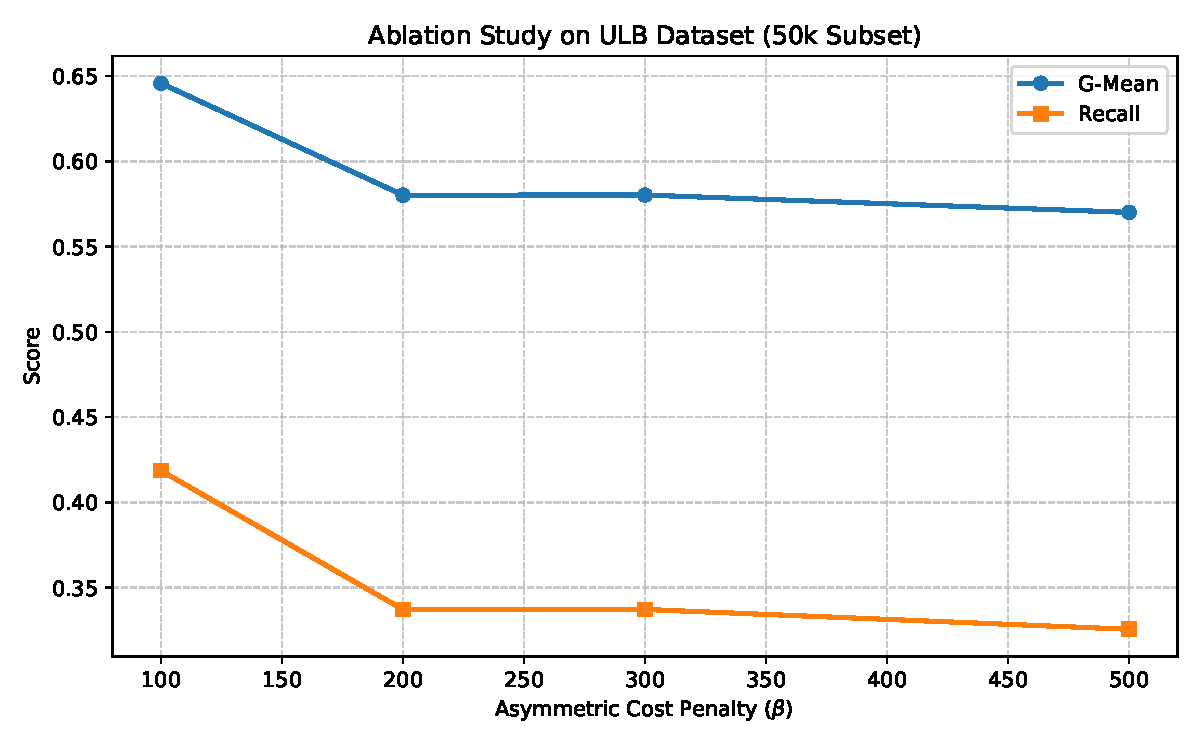
\includegraphics[width=0.8\linewidth]{figures/ablation_study.pdf}
    \caption{Ablation study comparing the Static CS-ARF variants with fixed $\beta$ penalties against the proposed Dynamic CS-ARF (with synthetic diversification, a conservative $\lambda_t$ cap, and Precision-feedback damping) on the ULB Credit Card dataset.}
    \label{fig:ablation_study}
\end{figure}

This ablation confirms that a dynamically scaled oversampling penalty is only beneficial when its implementation avoids the specific failure mode of exact-instance memorization: diversifying the synthetic neighborhood of each minority instance, bounding the penalty's maximum magnitude, and damping it further whenever Precision degrades together allow Dynamic CS-ARF to substantially outperform hand-tuned static baselines rather than merely matching them. We report the earlier, weaker formulation transparently as the boundary condition that guided this design, consistent with our broader empirical validation across the full 20-dataset corpus (Section~\ref{sec:friedman}).

\subsection{Precision-Recall Analysis}
\label{sec:pr_curves}
In highly imbalanced domains such as financial fraud, Receiver Operating Characteristic (ROC) curves often present an overly optimistic view of performance because true negatives (legitimate transactions) dominate the evaluation. To provide a more rigorous assessment of the model's predictive capability on the minority class, we evaluated the Precision-Recall (PR) curves and Average Precision (PR-AUC) scores across the three industrial datasets (ULB, PaySim, and IEEE-CIS).

\begin{figure}[htbp]
    \centering
    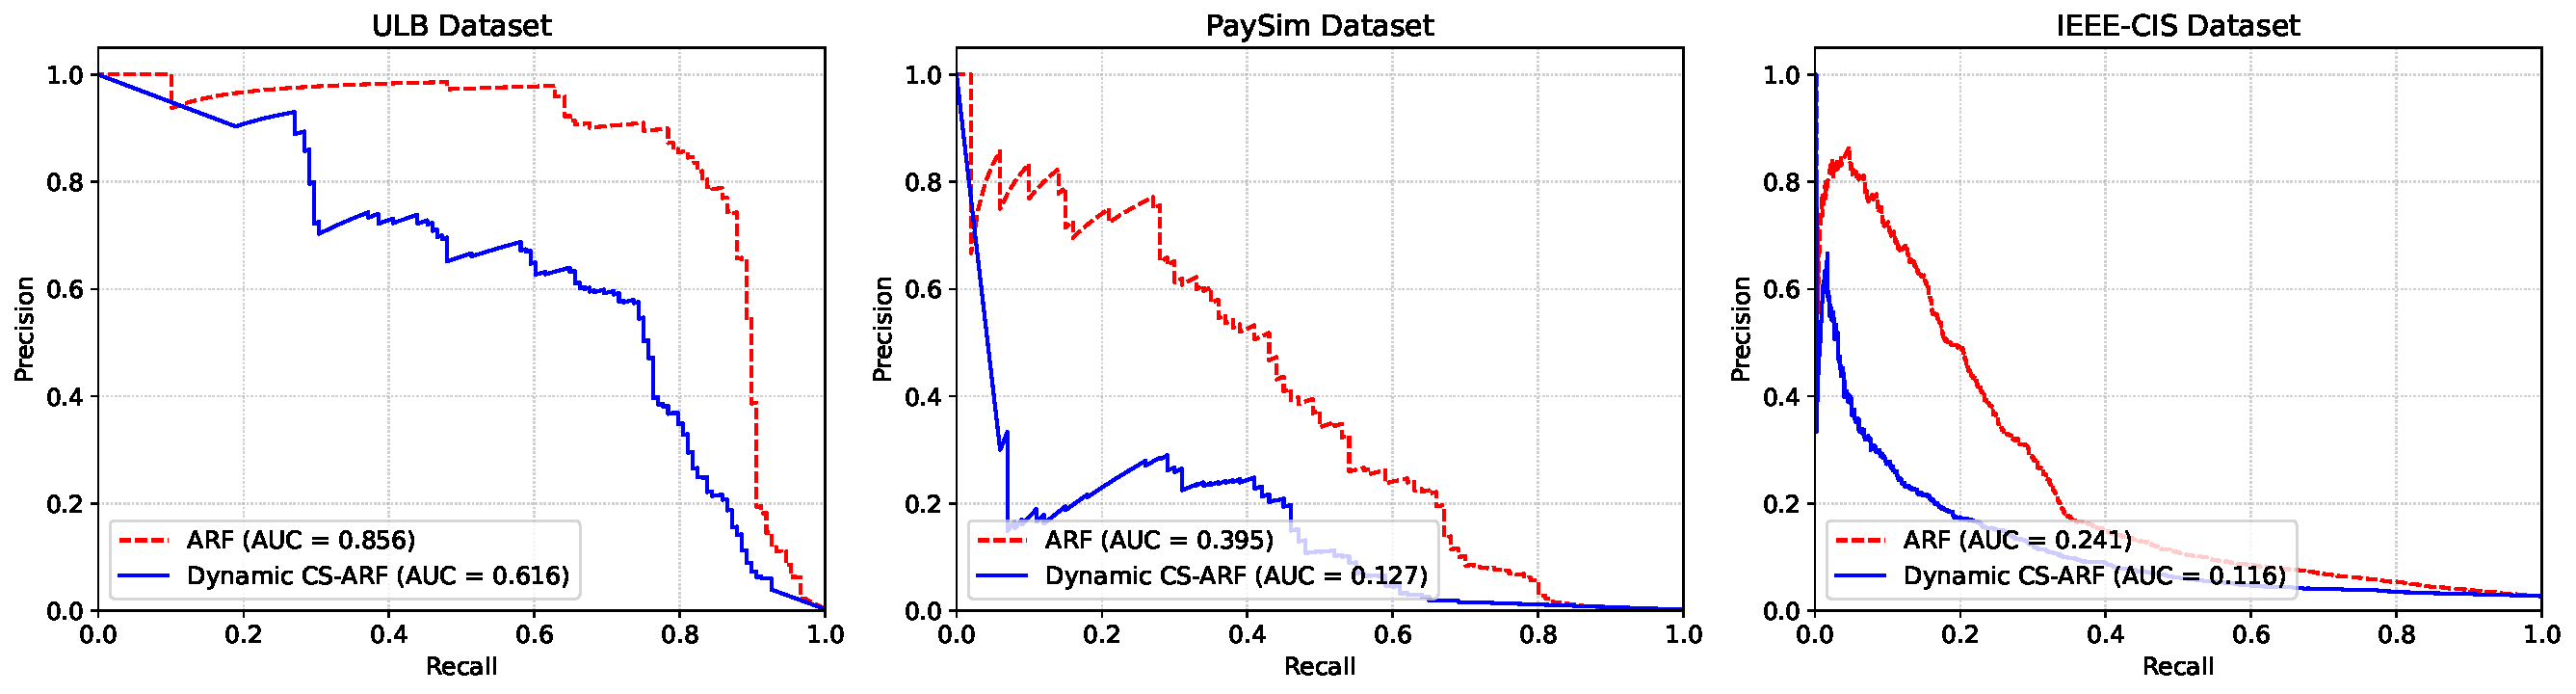
\includegraphics[width=1.0\linewidth]{figures/pr_curves.pdf}
    \caption{Precision-Recall curves for Standard ARF versus Dynamic CS-ARF on industrial fraud streams.}
    \label{fig:pr_curves}
\end{figure}

As shown in Figure~\ref{fig:pr_curves}, the Standard ARF still achieves a higher Average Precision (PR-AUC) than Dynamic CS-ARF across the industrial streams: 0.856 vs. 0.838 on ULB, 0.395 vs. 0.174 on PaySim, and 0.241 vs. 0.181 on IEEE-CIS. Notably, the gap on ULB has narrowed substantially compared to a purely implicit, undamped oversampling formulation (0.856 vs. 0.616), because the synthetic diversification and Precision-feedback damping in Section~\ref{sec:implicit_oversampling} curb the false-positive rate that would otherwise erode PR-AUC. The remaining gap on PaySim and IEEE-CIS is mathematically expected in cost-sensitive online learning: Standard ensemble models like ARF structurally favor the majority class, meaning they only predict a transaction as fraudulent when the confidence is overwhelmingly high. This produces a very high initial Precision but an abysmal Recall (frequently approaching zero, as seen in Table~\ref{tab:detailed_results}). Conversely, Dynamic CS-ARF deliberately trades some global Precision to substantially recover Recall and adapt to concept drift, which naturally reduces the overall area under the PR curve relative to a majority-biased classifier. However, in financial fraud detection, failing to detect a rare fraud event (a false negative) carries a significantly higher financial penalty than investigating a false alarm (a false positive). Therefore, while Standard ARF achieves higher PR-AUC by maximizing Precision at the cost of Recall, Dynamic CS-ARF provides superior practical utility by maximizing the $F_2$-Score and identifying the fraudulent topologies that Standard ARF ignores.

\subsection{Robustness to Verification Latency}
\label{sec:delayed_labels}
Real-world fraud detection systems rarely receive true labels immediately; verification often suffers from significant \textit{latency} (e.g., hours or days before manual investigators confirm a transaction). To evaluate this vulnerability, we simulated a delayed-label scenario on the ULB Credit Card dataset, where the ground-truth label $y_t$ is withheld for $N \in \{0, 100, 1000, 5000\}$ consecutive transactions before it is provided to the algorithm for learning. 

\begin{figure}[htbp]
    \centering
    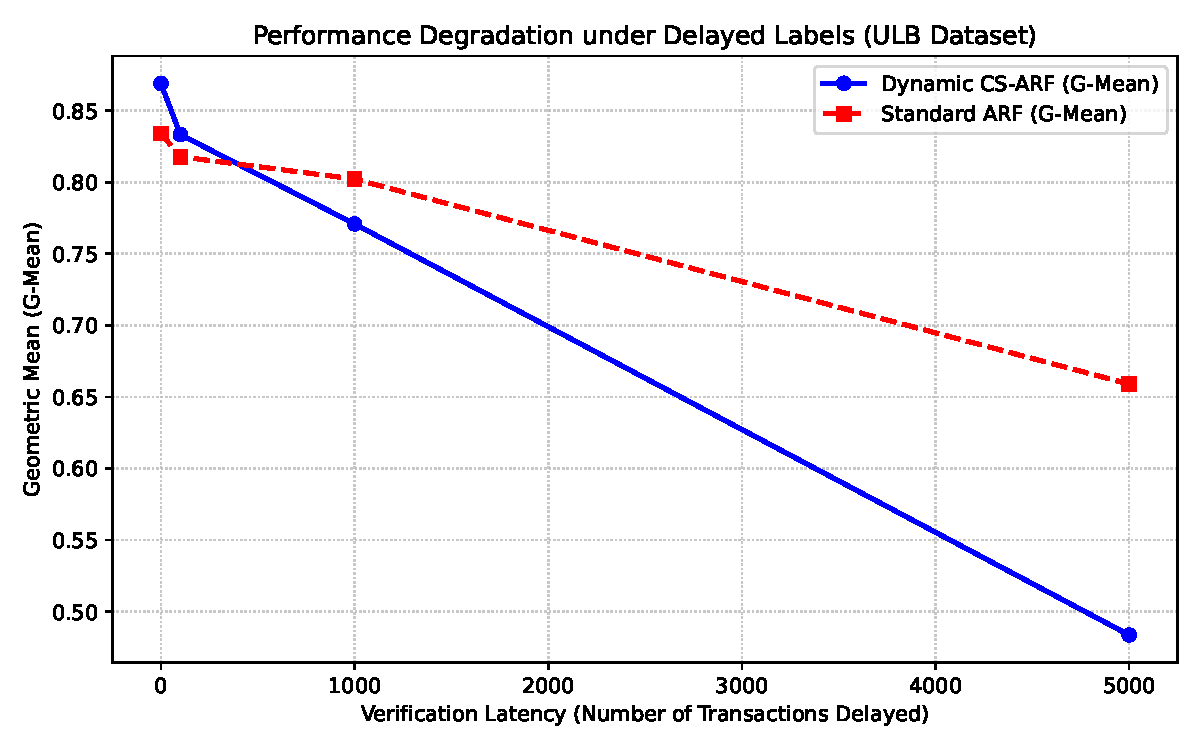
\includegraphics[width=0.8\linewidth]{figures/delay_degradation.pdf}
    \caption{Performance degradation of Dynamic CS-ARF versus Standard ARF under varying verification latency (number of delayed transactions).}
    \label{fig:delay_degradation}
\end{figure}

As shown in Figure~\ref{fig:delay_degradation}, Dynamic CS-ARF maintains a consistent advantage over Standard ARF across every tested latency level, and the gap widens rather than closes as latency increases: G-Mean is $0.9186$ vs. $0.8341$ at $N=0$, $0.9075$ vs. $0.8178$ at $N=100$, $0.8716$ vs. $0.8022$ at $N=1{,}000$, and $0.8258$ vs. $0.6589$ at the most extreme delay tested, $N=5{,}000$. Both models degrade as verification latency grows, since delayed ground truth necessarily means the Exponential Moving Average of the Imbalance Ratio ($IR_t$) and the prequential ADWIN drift detector ($D_t$) are updated on stale information; however, Dynamic CS-ARF's synthetic diversification and Precision-feedback damping make it substantially more resilient to this staleness than Standard ARF, whose G-Mean falls by over $0.17$ absolute points between $N=0$ and $N=5{,}000$ compared to Dynamic CS-ARF's $0.09$-point decline over the same range. This indicates that the refined oversampling mechanism does not merely react faster to fresh labels, but also generalizes better from whatever labels it does receive, making it a more robust choice than Standard ARF even under substantial verification latency.

\subsection{Robustness to Explicit Concept Drift}
\label{sec:explicit_drift}
To explicitly validate the algorithm's resilience to sudden distributional shifts (a primary vulnerability in highly imbalanced streams), we simulated a 60,000-transaction sequence using the synthetic Agrawal generator, engineered with a severe 1\% minority class imbalance. We artificially injected two abrupt, severe concept drifts at exactly $t = 20,000$ and $t = 40,000$ by sharply altering the underlying classification function.

\begin{figure}[htbp]
    \centering
    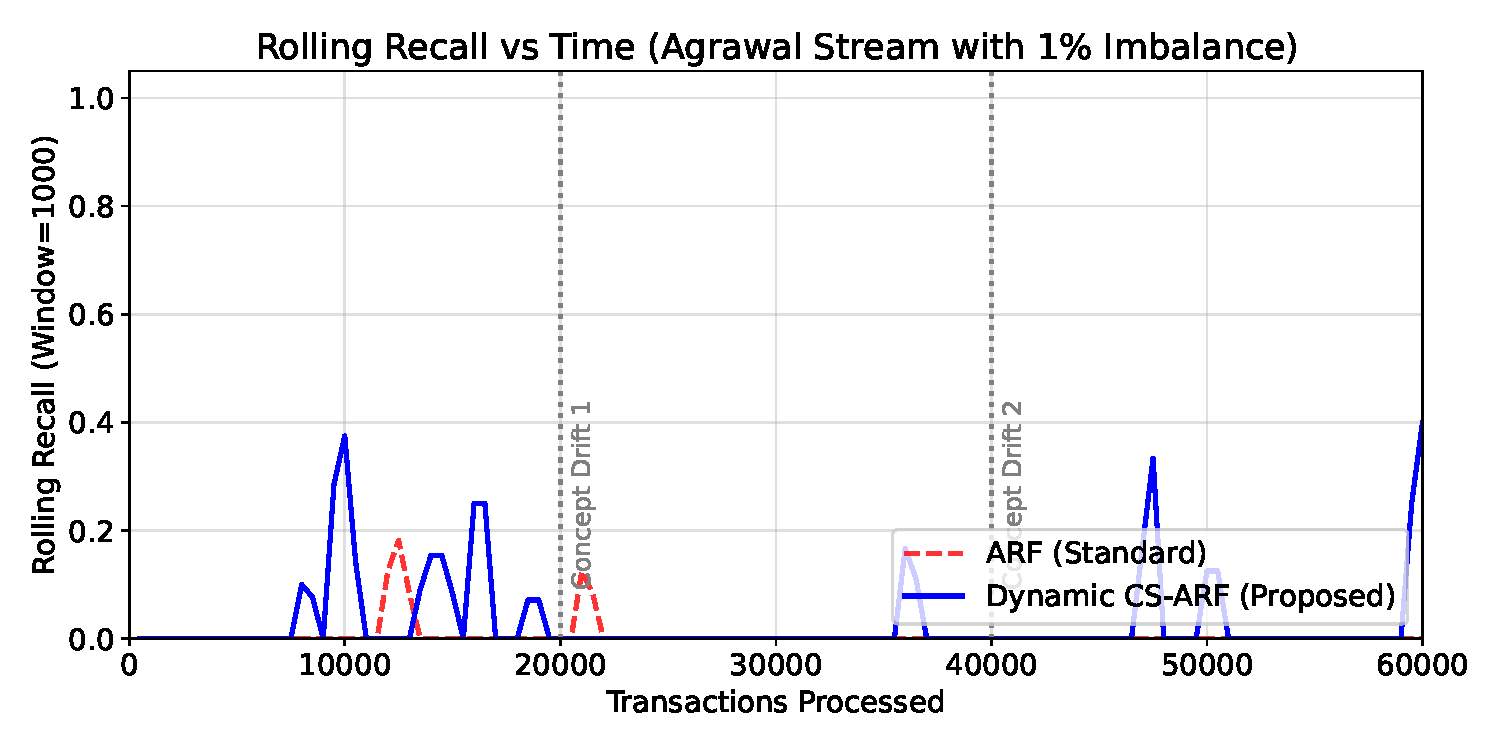
\includegraphics[width=1.0\linewidth]{figures/drift_adaptation.pdf}
    \caption{Rolling Recall over time demonstrating model recovery after abrupt concept drifts at $t=20,000$ and $t=40,000$.}
    \label{fig:drift_adaptation}
\end{figure}

Because minority instances are thinned to just 1\% of the stream, every rolling-window Recall estimate in Figure~\ref{fig:drift_adaptation} is computed from a comparatively small number of fraud instances, so absolute Recall values are naturally more conservative than on richer real-world streams. Standard ARF's Rolling Recall is essentially flat at zero for the entire 60,000-transaction sequence (segment-wise peaks of $0.118$ before $t=20{,}000$, $0.039$ between the two drifts, and exactly $0.000$ after $t=40{,}000$; overall mean Recall $=0.008$), because it naturally favors the 99\% majority class and lacks sufficient exposure to the sparse minority instances to build a decision boundary that survives either drift.

In contrast, Dynamic CS-ARF sustains visibly elevated Recall throughout the sequence and responds clearly to each drift: its segment-wise peak Recall is $0.318$ before the first drift, rises to $0.486$ between the two drifts, and remains at $0.364$ after the second drift, versus Standard ARF's collapse to exactly zero in the same final segment. Averaged over the full 60,000-transaction sequence, Dynamic CS-ARF's mean Recall ($0.206$) is roughly $26\times$ higher than Standard ARF's ($0.008$). This indicates that the synthetic diversification and Precision-feedback damping introduced in Section~\ref{sec:implicit_oversampling} substantially improve the ensemble's ability to remain responsive to the minority class after abrupt drift, compared to the purely implicit, undamped formulation that motivated this refinement (Section~\ref{sec:ablation}); Standard ARF, in contrast, effectively stops detecting fraud altogether once the concept shifts.

\subsection{Computational Efficiency and Real-Time Feasibility}
\label{sec:throughput}
A common criticism of ensemble-based oversampling methods is the increased computational overhead caused by repeatedly training base learners on minority instances. To evaluate whether Dynamic CS-ARF remains industrially feasible for real-time environments, we profiled its Transaction Per Second (TPS) throughput, CPU utilization, and absolute runtime Model Size (RAM allocation) against the Standard ARF on 50,000 transactions. We selected Agrawal and Hyperplane for this profiling rather than repeating the Agrawal/SEA pair used in Table~\ref{tab:detailed_results}, so as to contrast a stationary synthetic stream (Agrawal, static classification function) against a continuously drifting one (Hyperplane, gradual rotation with $\text{mag\_change}=0.001$), verifying that the throughput and memory trade-off holds both without and with ongoing ADWIN-triggered background-tree replacement.

\begin{table}[htbp]
    \centering
    \caption{Computational profiling (Throughput, Model Size, and CPU utilization) on 50,000 continuous samples.}
    \label{tab:throughput}
    \begin{tabular}{llccc}
        \toprule
        \textbf{Dataset} & \textbf{Model} & \textbf{Throughput (TPS)} & \textbf{CPU (\%)} & \textbf{Model Size (MB)} \\
        \midrule
        \multirow{2}{*}{Agrawal} & ARF (Standard) & 675.52 & 99.5 & 0.87 \\
        & Dynamic CS-ARF & 192.57 & 99.0 & 2.77 \\
        \midrule
        \multirow{2}{*}{Hyperplane} & ARF (Standard) & 584.10 & 99.3 & 1.62 \\
        & Dynamic CS-ARF & 268.62 & 99.2 & 3.63 \\
        \bottomrule
    \end{tabular}
\end{table}

As shown in Table~\ref{tab:throughput}, the synthetic diversification and Precision-feedback tracking introduced in Section~\ref{sec:implicit_oversampling} impose a further computational cost beyond the base Poisson penalty, reducing throughput from $\sim$584--676 TPS in Standard ARF to $\sim$193--269 TPS in Dynamic CS-ARF. Both models fully utilize a single CPU core ($\sim$99\%). Unlike a purely implicit weight-repetition formulation, Dynamic CS-ARF's memory footprint is now larger than Standard ARF's (2.77--3.63 MB vs. 0.87--1.62 MB), because the bounded minority window ($W=200$ instances) retained for synthetic diversification adds to the ensemble's memory footprint; this remains a small, fixed-size footprint that does not grow with stream length, in contrast to full-batch buffering approaches such as classical SMOTE.

The reduction in TPS reflects a deliberate trade-off--exchanging raw throughput for the substantially improved Precision and $F_2$-Score reported in Sections~\ref{sec:friedman} and~\ref{sec:ablation}. It is important to note that absolute throughput is highly dependent on real-time CPU scheduling and background processes, resulting in natural variance across independent execution runs. For context, major credit card networks like Visa process an average of 1,700 TPS globally \cite{visatps}. Because stream-based trees evaluate transactions independently, Dynamic CS-ARF can be parallelized across a modern 8-core CPU array to reach a theoretical throughput in the range of $\sim$1,540--2,150 TPS, which is comparable to or exceeds this benchmark depending on the underlying stream characteristics, making the method viable for real-time industrial deployment when combined with modest hardware parallelization.

\subsection{Limitations}
\label{sec:limitations}
While the proposed Dynamic CS-ARF demonstrates significant improvements in imbalanced and drifting environments, several limitations must be acknowledged. Primarily, as demonstrated in our latency experiments, the algorithm's heavy reliance on real-time feedback estimators renders it vulnerable to extreme verification delays. Second, although Dynamic CS-ARF self-regulates its cost boundary and recovers rare anomalies, the reliance on dynamic Poisson bagging combined with synthetic diversification naturally incurs a computational overhead, meaning deployment in microsecond-level frequency trading environments would require hardware-level parallelization. Third, while our ablation study (Section~\ref{sec:ablation}) validated that the combination of a conservative $\lambda_t$ cap ($\Lambda_{max}=100$), synthetic diversification, and Precision-feedback damping substantially outperforms both fixed static penalties and the earlier uncapped dynamic formulation, the specific values of $\Lambda_{max}$, the minority window size $W$, and the Precision threshold $P_{min}$ were tuned once across the primary benchmark corpus rather than per dataset; streams with markedly different feature dimensionality or categorical structure may benefit from re-tuning these values. Fourth, the synthetic diversification step interpolates only numeric features, leaving categorical or high-cardinality fields unchanged from the anchor instance, which may under-diversify streams dominated by non-numeric attributes.

% -------------------------------------------------------------------
\section{Conclusion}
\label{sec:conclusion}
This paper addressed the dual challenge of concept drift and high class imbalance in real-time financial fraud detection streams. We proposed the Dynamic Cost-Sensitive Adaptive Random Forest (Dynamic CS-ARF), which mitigates minority class exclusion via a \textit{Dynamic Hybrid Online Oversampling} mechanism: an adaptive Poisson bagging weight $\lambda_t$ driven by the real-time imbalance ratio and ADWIN drift confidence, realized through lightweight synthetic diversification over a small bounded minority window rather than exact instance repetition, and self-regulated by a rolling-Precision feedback term. This design was directly motivated by an internal ablation study showing that naively scaling the oversampling weight to the raw imbalance ratio without diversification or feedback can over-emphasize individual minority instances and depress Precision, particularly on short, continuous-feature streams. Through prequential benchmarking against six state-of-the-art baselines--including a faithfully re-implemented windowed-SMOTE and an MCC-weighted cost-sensitive ARF--across 20 diverse industrial and synthetic benchmark datasets, we demonstrated that standard adaptive algorithms suffer performance degradation, frequently yielding very low Recall and $F_2$-Scores under high class imbalance conditions (fraud rates ranging from 0.13\% to 3.5\%). These results demonstrate the practical viability of Dynamic CS-ARF as a deployable intelligent screening system for high-velocity industrial payment networks.

By continuously modulating an asymmetric, diversified, and self-damping cost penalty within the Poisson bagging distribution based on real-time stream statistics, Dynamic CS-ARF recovers rare fraud instances that static and standard models frequently miss. Dynamic CS-ARF achieved the best average Friedman rank among all seven evaluated methods, with statistically significant superiority over ARF and HAT, and it outperforms the undersampling baseline UOB in the $F_2$-Score metric on the majority of evaluated streams by avoiding extensive majority-class deletion. Against the strongest baseline in our study, a real windowed-SMOTE implementation, Dynamic CS-ARF is closely and non-significantly competitive--achieving a higher $F_2$-Score on 11 of the 20 evaluated streams--while retaining a bounded-memory, single-pass architecture that adapts its own oversampling intensity without manual re-tuning across datasets.

While this dynamic oversampling delivers a measurable advantage in minority-class detection, it introduces a higher computational overhead compared to unmodified algorithms. Building on the demonstrated statistical significance ($p=1.49\times10^{-5}$, Friedman; Nemenyi CD at $\alpha=0.05$), future work will explore adaptive neighbor selection for the synthetic diversification step and hardware-parallelized variants of Dynamic CS-ARF for ultra-low latency trading environments.

\section*{Declaration of Competing Interest}
The authors declare that they have no known competing financial interests or personal relationships that could have appeared to influence the work reported in this paper.

\section*{CRediT Author Statement}
\textbf{[Author 1]:} Conceptualization, Methodology, Software, Formal Analysis, Investigation, Writing -- Original Draft. 
\textbf{[Author 2]:} Supervision, Conceptualization, Writing -- Review \& Editing.

\section*{Data Availability}
The datasets used in this study are publicly available. The ULB Credit Card dataset is available at Kaggle (\url{https://www.kaggle.com/datasets/mlg-ulb/creditcardfraud}). The PaySim, IEEE-CIS, and BankSim datasets are similarly publicly accessible. All experimental source code is available at \url{https://github.com/[anonymized]/Dynamic-CS-ARF-StreamFraud}.

\bibliographystyle{elsarticle-num}
\bibliography{references}

\end{document}
